\documentclass{rapport}
\usepackage[utf8]{inputenc}

\usepackage{pifont} % Pour les symboles appelés par la macro \ding
\usepackage{url} % Comme son nom l'indique, pour les url...

\usetikzlibrary{positioning} % Bibliothèque tikz pour positionner des nœuds relativement à d'autres

\usepackage[colorlinks, citecolor=red!60!green, linkcolor=blue!60!green, urlcolor=magenta]{hyperref} % Pour que les liens soient cliquables. Les options permettent de mettre les liens en couleur.

\usepackage{algorithm}
\usepackage{algo}
\usepackage{colorationSyntaxique}
\usepackage{listings}
\usepackage{graphicx}
\usepackage{float}


% Pour un rapport en français 
% \usepackage[francais]{babel} % Commenter pour un rapport en anglais
% \renewcommand\bibsection{\section*{Bibliographie}} % Commenter pour un rapport en anglais

\englishTitlePage % Décommenter pour une page de titre en anglais


\pagestyle{fancy}
\renewcommand{\sectionmark}[1]{\markboth{\thesection.\ #1}{}}
\fancyfoot{}

\newcommand{\gcc}{\texttt{gcc} }
\newcommand{\icx}{\texttt{icx} }
\newcommand{\clang}{\texttt{clang} }
\newcommand{\comp}{\texttt{ccomp} }
\newcommand{\optizero}{\texttt{-O0} }
\newcommand{\optione}{\texttt{-O1} }
\newcommand{\optitwo}{\texttt{-O2} }
\newcommand{\optithree}{\texttt{-O3} }
\newcommand{\optisize}{\texttt{-Os} }

\fancyhead[LE]{\textsl{\leftmark}}
\fancyhead[RE, LO]{\textbf{\thepage}}
\fancyhead[RO]{\textsl{\rightmark}}

\def\Latex{\LaTeX\xspace}
\def\etc{\textit{etc.}\xspace}

\lstset{                  % Specify language
basicstyle=\ttfamily\small,     % Code font and size
keywordstyle=\color{blue},      % Color for keywords
commentstyle=\color{gray},      % Color for comments
stringstyle=\color{red},        % Color for strings
numbers=left,                   % Add line numbers
numberstyle=\tiny\color{gray},  % Style for line numbers
% frame=single,                   % Add a border around code
breaklines=true,                % Line wrapping
% backgroundcolor=\color{gray!10} % Light gray background
}


\title{Optimizing application performance through optimizing compilation}
\author{Francois Flandin}
\supervisor{Pr Sid Touati}
\date{First semester of year 2024-2025}

% \universityname{Université Côte d'Azur} % Nom de l'université.
% \type{TER} % Type de document
% \formation{Master Informatique} % Nom de la formation

% Retrouver les autres options possibles dans le document rapport.pdf

\begin{document}

\maketitle

\begin{abstract}

\end{abstract}

\clearpage
\tableofcontents

\clearpage
\section{Introduction}
The tutorship project "Optimizing application performance through optimizing compilation" consists of studying how compilers optimize the generated code with their options \optizero, \optione, \optitwo, \optithree, \optisize, and how efficient the generated code is.
\newline
There are 2 steps to the project,
\begin{itemize}
\item First, take two programs (shown in the second part), compile them with 4 compilers which are \gcc, \icx, \clang, and \comp, and with each compilers, all the optimizations levels.
Then we calculate how much time it takes to execute each 20 programs, we calculate the mean over 12 executions.
\item Then, study for each compiler which optimizations options are enabled with each optimization levels.
\end{itemize}
\clearpage

\part{The experience}

\section*{Experience's environnement}
In this part will be presented the environnement of the experimentations, on which hardware it was done, on which software, etc.
\subsection*{Hardware}
In this part, the hardware part of the computer will be explored. \newline
To explore the hardware of a computer on linux, the folder \texttt{/cpu} can be explored, it gives us the \textit{topology} of the cpu, like which threads are on each cores, which caches are on each cores, discover what is the cache line size etc...\newline
But there are also a lot of linux tools that allows to check the hardware's specifications of a computer, and basically doing the job for us. \newline
There are graphical tools such as \texttt{likwid}, which provides the command \texttt{likwid-topology}, or the tool \texttt{hwloc}, which provides \texttt{lstopo}, a command that gives a beautiful GUI of the computer's hardware's specification.
\begin{description}
    \item[Model name :] 11th Gen Intel(R) Core(TM) i5-1135G7 @ 2.40GHz
    \item[Adress size :] 39 bits physical, 48 bits virtual
    \item[Cache line size :] 64 bytes
    \item[Cores :] 4
\end{description}

\begin{table}[H]
    \centering
    \begin{tabular}{|l|c|c|c|c|}
        \hline
        \multicolumn{5}{|c|}{Graphical Topology} \\
        \hline
        Coeurs & \enspace0\enspace\enspace4 &\enspace1\enspace\enspace5 &\enspace2\enspace\enspace6 &\enspace3\enspace\enspace7 \\
        \hline
        Cache L1 & \enspace48 kB &\enspace48 kB &\enspace48 kB &\enspace48 kB \\
        \hline
        Cache L2 & 1MB & 1MB & 1MB & 1MB \\
        \hline
        Cache L3 & \multicolumn{4}{|c|}{8 MB} \\
        \hline
    \end{tabular}
    \caption{Computer's topology}
    \label{tab:graph_characteristics}
\end{table}


\subsection*{Software}
For the software part, the experiments were done on a lightweight configuration of the computer, where all unnecessary services were disabled, including the graphical interface, this allows the computer to run as baremetal as possible. \newline
Here is a description of all the software elements used in this benchmark :
\begin{description}
    \item[OS] Fedora Linux v40 WorkStation
    \item[gcc] version 14.2.1 20240912
    \item[icx] version 2024.2.1.20240711
    \item[clang] version 18.1.8
    \item[ccomp] version 3.14
\end{description}


\section{Results}
\begin{figure}[H]
\centering
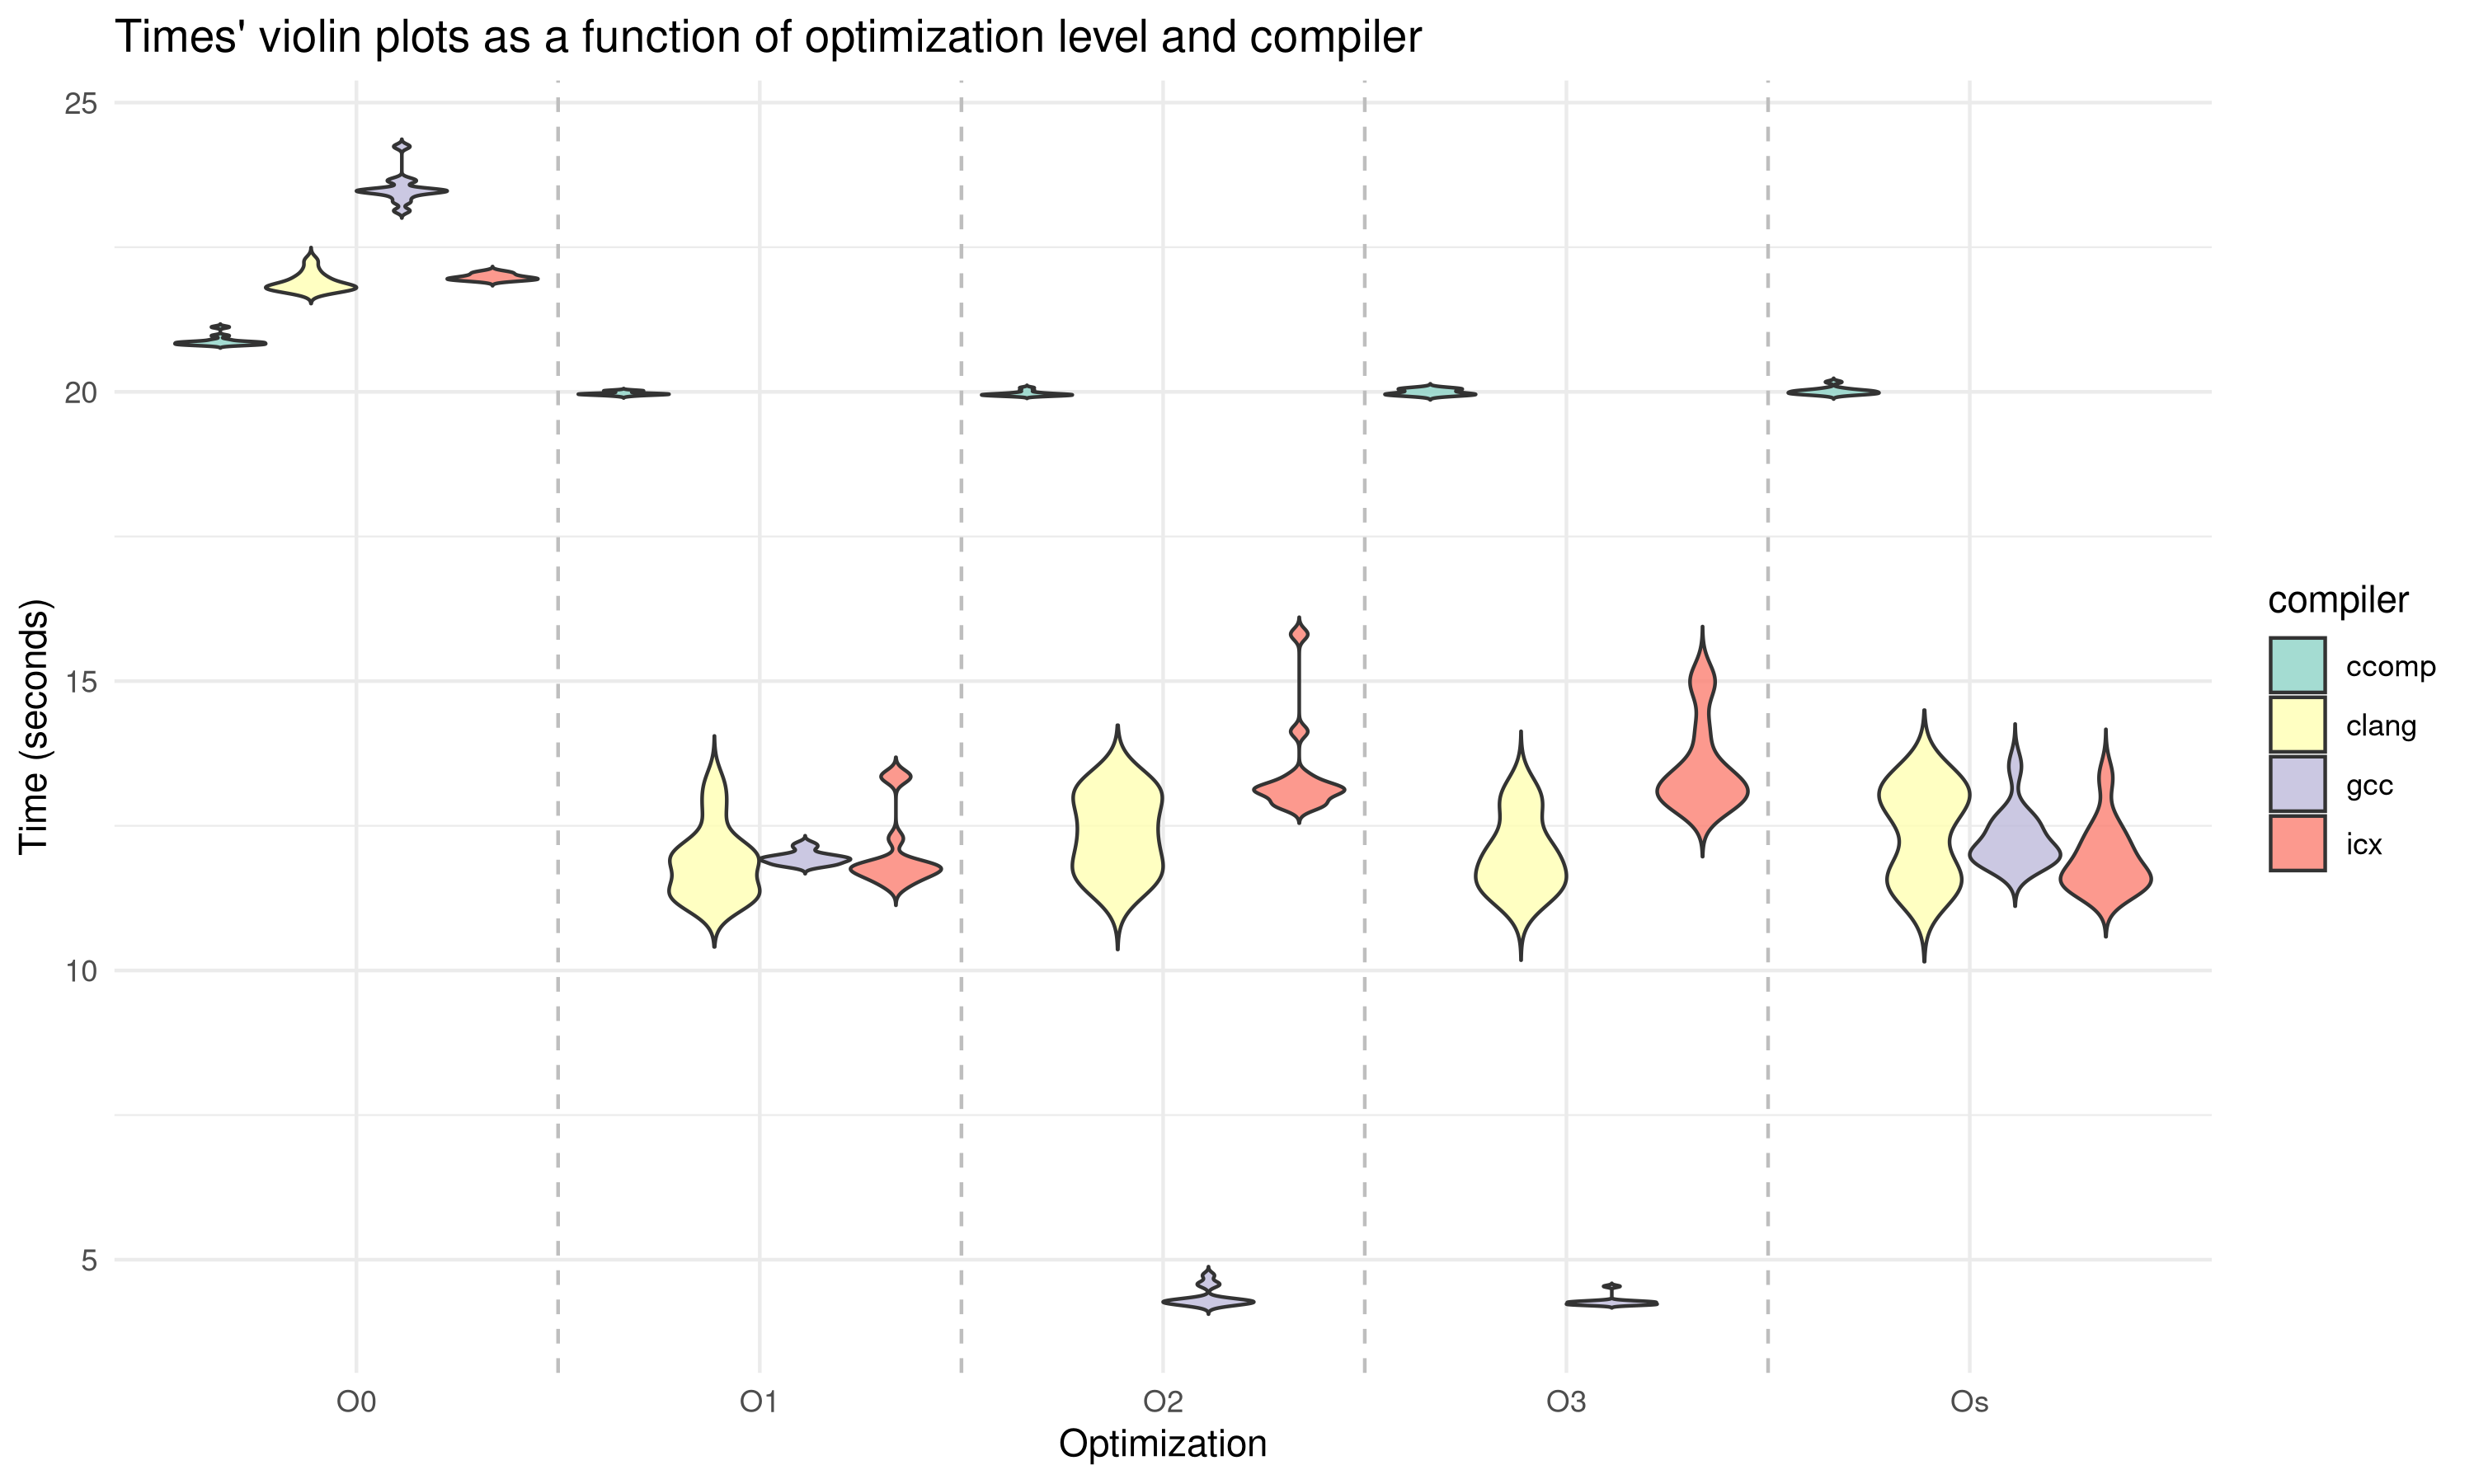
\includegraphics[width=1\textwidth]{img/plots/violin_plot_mat_mult.png}
\caption{Evolution of the execution time of the program mat\_mult.c as a function of compiler and optimization level.}
\label{fig:image1}
\end{figure}
What we notice here is that \gcc gives the most optimized programs of them all, even by starting as the worst one, \comp is the worst one and can even notice that its execution times are really constant, the violin plots looks the same across all optimizations. \newline
\icx and \clang doesn't offer good performance when comparing to \gcc, but still offers good optimisation.


\begin{figure}[H]
\centering
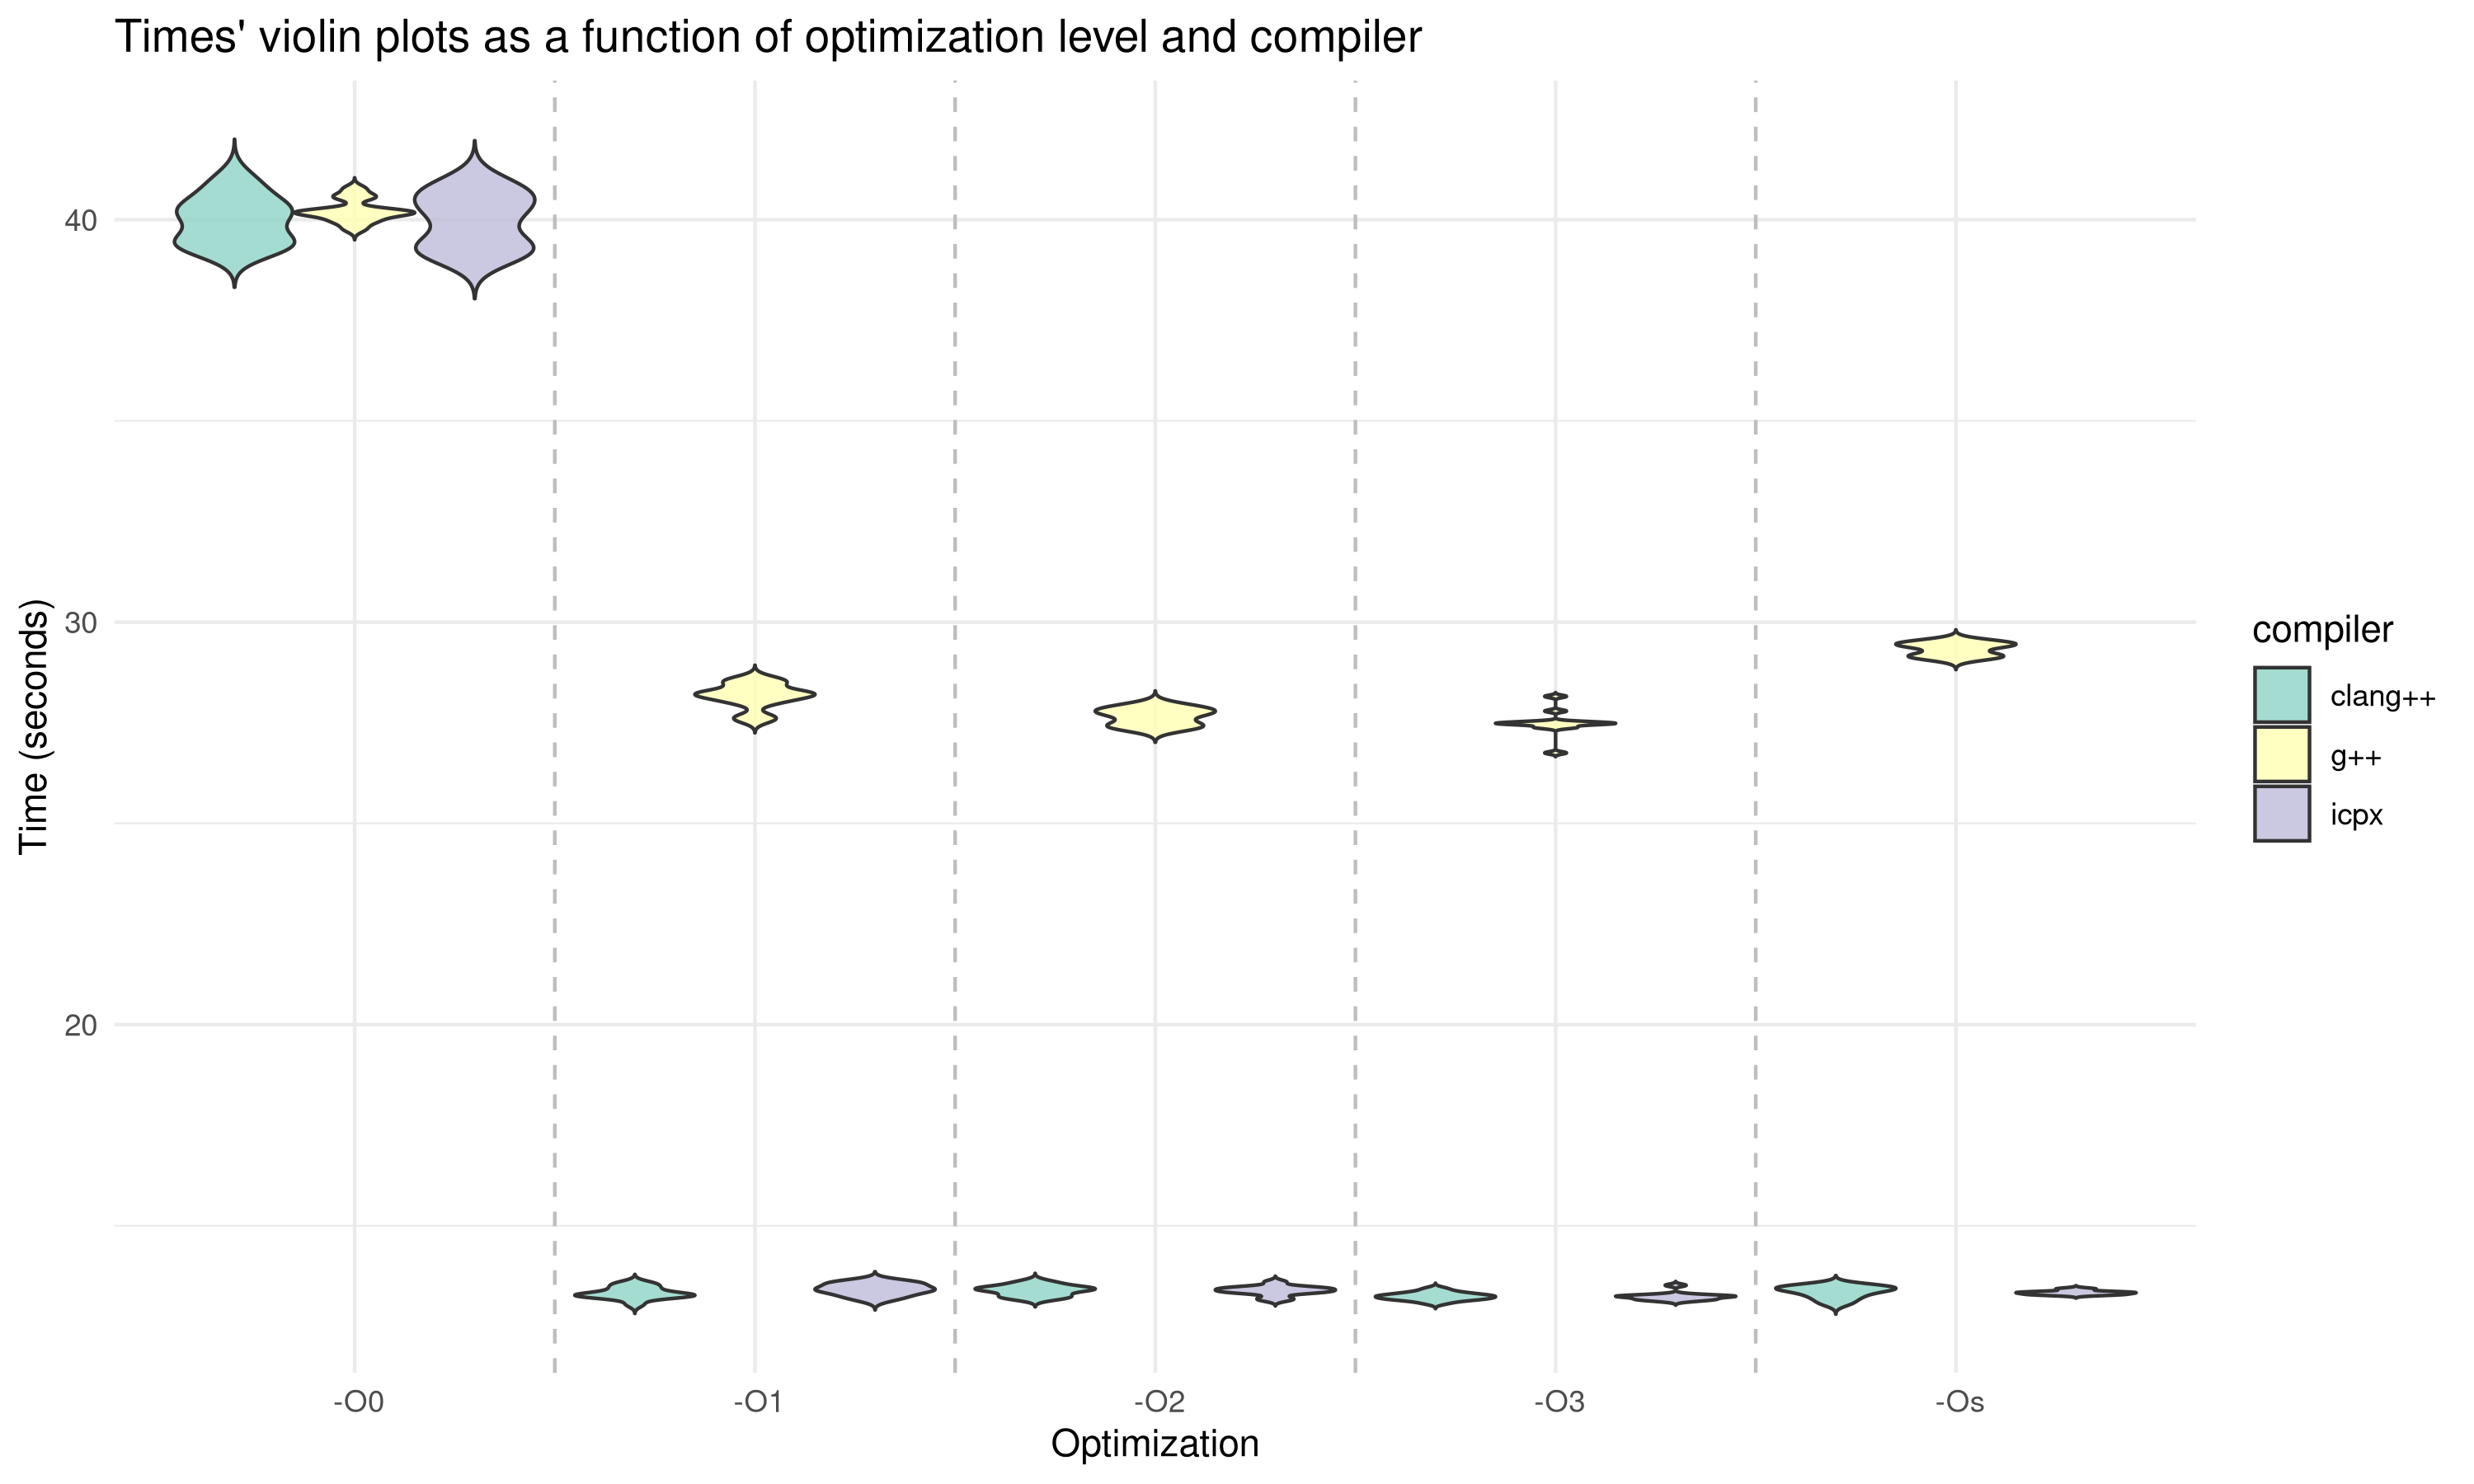
\includegraphics[width=1\textwidth]{img/plots/violin_plot_dijkstra.png}
\caption{Evolution of the execution time of the program dijkstra.cpp as a function of compiler and optimization level.}
\label{fig:image2}
\end{figure}


\clearpage
\part{Compilers}
In this part will be presented all the compilers used in this tutorship project, as well as deepening their optimization options for each optimizations levels.
\section{\gcc}
\gcc is the most popular \texttt{C} compiler, it comes in the \texttt{GNU Compiler Collection}, which includes compilers for \texttt{Fortran}, \texttt{C++}, \texttt{Go}...
\subsection{Optimization options}
\subsubsection{Options introduced by \optizero}
\gcc \optizero was originally meant to disable every optimization flags to give the least optimized code, however, the competition with other compilers led to now have some optimization flags enabled, 53 to be more precise. Here are some of the most important ones:
\newline
\begin{description}
    \item[Loop optimizations] with the option \texttt{-faggressive-loop-optimizations}, \gcc enables, as its name suggests, a lot of loop optimizations, such as \textbf{loop fusion} and \textbf{fission}, \textbf{loop unrolling}, \textbf{loop peeling}.
    \item[Dead Code elimination] \gcc can also remove every line of code that isn't used, this doesn't impact the execution speed, but reduces the size of the generated code.
    \item[Peephole optimizations] This option introduces optimizations on the operators, for example a common optimization would replace $a*2$ with $a<<1$. It also reduces the redundant register moves.
\end{description}
Other enabled options at \optizero are either analysis options or add error-handling instructions.

\subsubsection{Options introduced by \optione}
\gcc \optione optimizations add optimizations to the tree that the compiler builds in the intermediate level, these optimizations include :
\newline
\begin{description}
    \item[Dead Code and Redundancy elimination] With the options \texttt{-ftree-dce}, \texttt{-ftree-fre} and \texttt{-ftree-dse}, \gcc removes all the \textbf{dead code}, computations that produce the same results as well as all \textbf{dead stores}, that means that the cpu has less operations to manage, and the code size is reduced.
    
    \item[Value and Copy propagation] First, the option \texttt{-ftree-ccp} tells the compiler to propagate constant values across conditions when it's possible, it simplifies all the control flow and makes place for further optimizations, and can even help for \texttt{branch prediction}. \newline Secondly, the option \texttt{-ftree-copy-prop} propagates values with copy instructions, for example \texttt{b = a; c = b;} would be replaced with \texttt{c = a;}.
    
    \item[Loop optimization] There are two main options here to consider, the first, \texttt{-ftree-sink} moves computations outside of the loop when it's possible, it allows to avoid computing the same thing over and over. \newline
    The second is \texttt{-ftree-sra} for \textit{scalar replacement of aggregates}, it breaks structures and array into individual variable when needed, it can improve register usage and enable even further optimizations. An example of this would be a variable of the struct \texttt{Point \{int x; int y\}} would be transformed from \texttt{Point p;} to \texttt{int p\_x, p\_y;}.
\end{description}
At \optione, there are also other options to enable inlining of functions, that means that a function call will be replaced by the function's body, which allows for further optimizations.


\subsubsection{Options introduced by \optitwo}
\gcc \optitwo introduces aligning of functions, jumps, labels, and loops, the aligning allows to ensures that the instructions fit at the beginning of cache lines, which can reduce cache misses. Also, aligning labels and jumps allows to decrease branch prediction misses.
\newline
\optitwo also enables \texttt{-funroll-loops}, which performs loop unrolling when iteration count is known, which allows the compiler to optimize as it wishes.


\subsubsection{Options introduced by \optithree}
\gcc \optithree enables also further loops optimizations, such as :

\begin{description}
    \item[Loop peeling] which removes special cases in the loop and put them outside of the loop.
    \item[Loop jamming] which combines two loops with the same scope/range into a single one, enabling more optimizations, it is generally combined with \texttt{loop unrolling}.
    \item[Loop interchange] allows the compiler to swap two loops in a nested loop, this allows to put the most changing variable to the consecutive elements in memory, instead of having the most changing variable to the separate elements in memory, it's very useful in programs such as \texttt{matrix multiplication}.
    \item[Loop splitting] allows simplification of a loop by dividing it into several loops, it simplifies the loops with the pattern \textbf{for (int $i=0$; $i<10$; $i++$) if($i<5$)... else} into two loops, one with the range 0..4 and the other 5..9. It help in reducing dependencies.
\end{description}

\subsubsection{Options enabled by \optisize}
\gcc \optisize enables the same options as \gcc \optitwo, but removes the aligning optimizations to free some space.






\section{\icx}
It's Intel's compiler for their x86 architecture.
\subsection{Optimization options}
\subsubsection{Options introduced by \optione}
At this level of optimization, \icx starts by introducing \textbf{data flow analysis}, to help gathering data about data flows throughout the whole program, allowing for optimizations.
Then, the compiler can also reorganize code as he wishes with \textbf{code motion}, which allows to move non-changing result operations out of loop to avoid recomputing it over and over, and \textbf{instruction scheduling}, which allows to change the order of instructions, to hide memory latency for exemple, or doing something while something heavier is done. It is done to reduce CPU stall.
\newline\newline
Other optimizations are also enabled, \textbf{strength reduction}, that changes heavy operations for cheaper ones, like switching from a multiplication to a bit shift, \textbf{test replacement}, that simplifies loops' conditions for example : 
\begin{verbatim}
    if (x >= 0 && x < 100) { /* code */ } // base loop
    if ((unsigned)x < 100) { /* code */ } // optimized loop
\end{verbatim}
And, finally, \textbf{split-lifetime analysis}, can split the \textit{lifetime} of a variable into smaller lifetimes, to reallocate the registers when the variable is not used anymore.

\subsubsection{Options introduced by \optitwo}
At this level of optimization, \icx introduces more optimizations, like \textbf{constant propagation}, or \textbf{forward substitution}, which can replace variable with their expressions, for example : 
\begin{verbatim}
    int a = 5 + i
    int b = a + 3
\end{verbatim}
will be replaced by
\begin{verbatim}
    int b = 5 + i + 3
\end{verbatim}
These two options complete each other really well, because imagine that the variable \texttt{i} was a constant, it would be replaced by its value, hence further optimizing the program.\newline\newline
Additionnal optimizations are introduced, like \textbf{loop unrolling}, which reduces the number of iterations by executing multiple iterations within a single loop cycle,\textbf{peephole optimizations}, which examines small code fragments to identify and replace inefficiencies, such as redundant instructions or suboptimal sequences, improving code quality. Or even \textbf{optimized code selection}, replaces inefficient instructions or code sequences with more efficient alternatives.
\newline\newline
There are also code-removing optimizations such as \textbf{dead-code elimination}, \textbf{dead-store elimination}, and \textbf{dead static function elimination} which does not really improves performance but can help reduce the weight put on the CPU.

\subsubsection{Options introduced by \optithree}
It enables all the same optimizations as \optitwo but add more aggressive loop transformations such as \textbf{loop fusion}, \textbf{block-unroll-and-jam}, with these two options, the compiler expands and find the best fusions/jams in the loops and \textbf{collapsing-IF-statements}, where multiple successive if are combined into one to reduce branching therefore gaining performances.

















\section{\comp}
\textit{Certified Compiler}\newline
It's the only C compiler that is mathematically verified to produce the code described by the source code. 
%In this part will be presented all the optimizations options that \comp enable at each optimization level, the only difference is that with this compiler, \optione, \optitwo and \optithree are all the same option, they enable the same optimizations. Moreover, \optizero enables nothing.
\subsection{Optimization options}
\comp doesn't enable anything at \optizero, and the main optimization level \texttt{-O} gives the same optimizations as \optione, \optitwo, \optithree, because they are just an alias of that optimization option.
\subsubsection{Options introduced by \optione/\optitwo/\optithree}
There are not a lot of options so here is a list of them

\begin{description}
    \item[-fcont-prop] enables constant propagation, a process that replaces variables with their known constant values throughout the program.
    \item[-fcse] activates the elimination of common subexpressions, reducing redundant calculations by reusing previously computed values.
    \item[-fif-conversion] with this option, the compiler decides whether to replace simple if-then-else statements or the conditional operator (?:) with conditional assignements.\newline
    The heuristic-based approach selectively optimizes small and balanced expressions, provided the target architecture supports a suitable conditional move instruction.
    \item[-finline]  enables or disables the inlining of functions, potentially improving performance by replacing function calls with the actual function code.
    \item[-finline-functions-called-once] specifically inlines functions that are called only once, reducing overhead while maintaining efficiency.
    \item[-fredundancy] activates the elimination of redundant computations and unnecessary memory stores, improving execution time by avoiding repetitive operations.
    \item[-ftailcalls] optimizes function calls in tail position, which can enhance performance by reusing the current function’s stack frame. 
    \item[-ffloat-const-prop 2] enables full propagation of floating-point constants, ensuring arithmetic is performed in IEEE double precision format with round-to-nearest mode.
\end{description}


\section{clang}
It's a compiler made by the LLVM Developer Group, it can replace \gcc by supporting most of the option flags of \gcc. \newline
The objective behind this compiler is to create a compiler that allowed: first, better diagnostics, which allows to debug more easily, second, to be seperated from the GNU licence, which forced
softwares to be integrated to said licence and therefore having to open\-source proprietary software, third, to have a nimble compiler that is simple and easy to develop and maintain.
\subsection{Options enabled at \optizero}
\clang like the other compilers doesn't enable a lot of optimizations, the optimizations are called \textbf{AlwaysInlinerPass}, which inlines functions marked
with the \texttt{always\_inline} attribute, \textbf{CoroConditionalWrapper}, which is related to coroutines support in C++ (aucune idee de ce que c'est faut vraiment
que je check), and finally \textbf{VerifierPass}, which ensures that the LLVM Intermediate Representation generated by the compiler is correct and coherent 
with the original program.

\subsection{Options enabled at \optione, \optitwo, \optithree}
Like for \comp, they enable all the same optimizations

%https://clang.llvm.org/

\clearpage
\nocite{*}
\bibliographystyle{plainnat}
\bibliography{bibliox}

\end{document}
